\documentclass[aspectratio=169]{beamer}
\usepackage[utf8]{inputenc}
\usepackage[T1]{fontenc}
\usepackage[brazil]{babel}
\usepackage{ragged2e}
\usepackage{booktabs}
\usepackage{verbatim}
\usepackage{gensymb}
\usepackage{multirow}
\usepackage{xcolor,colortbl}
\definecolor{verde}{rgb}{0,0.5,0}
\usepackage{listings}

\lstset{language=C++,
	backgroundcolor=\color{green!10},
	basicstyle=\ttfamily,
	keywordstyle=\color{blue}\ttfamily,
	stringstyle=\color{red}\ttfamily,
	commentstyle=\color{green}\ttfamily,
	morecomment=[l][\color{magenta}]{\#},
	literate=
	{á}{{\'a}}1
	{à}{{\`a}}1
	{ã}{{\~a}}1
	{â}{{\^a}}1
	{é}{{\'e}}1
	{ê}{{\^e}}1
	{í}{{\'i}}1
	{ó}{{\'o}}1
	{õ}{{\~o}}1
	{ú}{{\'u}}1
	{ü}{{\"u}}1
	{ç}{{\c{c}}}1
	{Á}{{\'A}}1
	{À}{{\`A}}1
	{Ã}{{\~A}}1
	{Â}{{\^A}}1
	{É}{{\'E}}1
	{Ê}{{\^E}}1
	{Í}{{\'I}}1
	{Ó}{{\'O}}1
	{Õ}{{\~O}}1
	{Ú}{{\'U}}1
	{Ü}{{\"U}}1
	{Ç}{{\c{C}}}1
}

\newcommand\setItemnumber[1]{\setcounter{enumi}{\numexpr#1-1\relax}}

\usetheme{AnnArbor}
\usecolortheme{orchid}
\usefonttheme[onlymath]{serif}

\AtBeginSection[]{
  \begin{frame}
  \vfill
  \centering
  \begin{beamercolorbox}[sep=8pt,center,shadow=true,rounded=true]{title}
    \usebeamerfont{title}\insertsectionhead\par%
  \end{beamercolorbox}
  \vfill
  \end{frame}
}

\title[\sc{Herança}]{Herança}
\author[Roland Teodorowitsch]{Roland Teodorowitsch}
%\institute[LP2 - EC - PUCRS]{Laboratório de Programação II - Curso de Engenharia de Computação - PUCRS}
\institute[POO - EC - PUCRS]{Programação Orientada a Objetos - ECo - Curso de Engenharia de Computação - PUCRS}
\date{29 de maio de 2024}

\begin{document}
\justifying

%-------------------------------------------------------
\begin{frame}
	\titlepage
\end{frame}

%=======================================================
\section{Herança}

%-------------------------------------------------------
\begin{frame}\frametitle{Herança}
\begin{itemize}
	\item Ao modelar um conjunto de classes, é possível encontrar classes semelhantes na estrutura e no comportamento
	\begin{itemize}
		\item Solução 1: modelar as classes de forma independente (duplicação de código)
		\item Solução 2: extrair características estruturais e comportamentais que sejam comuns e colocá-las em classes mais gerais a partir das quais são definidas classes mais específicas (\textbf{herança})
	\end{itemize}
\end{itemize}
\end{frame}

%-------------------------------------------------------
\begin{frame}\frametitle{Herança}
\begin{itemize}
	\item É a propriedade da programação orientada a objetos que permite expressar o compartilhamento de características comuns entre as classes
	\item Permite a reutilização de código através especialização de soluções genéricas já existentes
\end{itemize}
\end{frame}

%-------------------------------------------------------
\begin{frame}[fragile]\frametitle{Sintaxe da Herança}
\begin{itemize}
	\item Em C++, pode-se criar uma classe \textbf{derivada} a partir de uma classe \textbf{base} usando:
\begin{lstlisting}[language=C++,basicstyle=\ttfamily\scriptsize]
class Base {
  // Membros
};

class Derivada : /* public, private, protected */ Base {
  // Outros membros
};
\end{lstlisting}
	\item O acesso aos membros da classe base será no máximo o definido na herança
	\item Se o modificador de acesso for omitido, será usado \textbf{\texttt{private}}
\end{itemize}
\end{frame}

%-------------------------------------------------------
\begin{frame}\frametitle{Aspectos da Herança}
\begin{itemize}
	\item Os seguintes aspectos devem ser considerados quando se usa herança:
	\begin{itemize}
		\item Acesso a Atributos e Métodos Privados
		\item Construtor
		\item Sobrescrita de Métodos
		\item Herança Múltipla
	\end{itemize}
\end{itemize}
\end{frame}

%-------------------------------------------------------
\begin{frame}[fragile]\frametitle{Acesso a Atributos e Métodos Privados}
\begin{itemize}
	\item Atributos e métodos privados na superclasse, usualmente, NÃO são acessíveis na subclasse. Assim, se:
\begin{lstlisting}[language=C++,basicstyle=\ttfamily\scriptsize]
class Aluno {
  private:
    int matricula;
    string nome;
  public:
    string obtemNome();
};
\end{lstlisting}
	\item E a herança for declarada usando \texttt{public}, deve-se usar a interface pública da classe base:
\begin{lstlisting}[language=C++,basicstyle=\ttfamily\scriptsize]
class AlunoRegular : public Aluno {
  ...
  string obtemNomeComPrefixo() {
    return "Aluno: " + obtemNome();
  }
};
\end{lstlisting}
\end{itemize}
\end{frame}

%-------------------------------------------------------
\begin{frame}\frametitle{Membros Protected}
\begin{itemize}
	\item A subclasse \textbf{herda} (tem acesso) apenas os métodos e atributos públicos da superclasse
	\item O acesso aos atributos privados deve ser feito através de métodos públicos
	\item É possível declarar atributos da superclasse como \texttt{protected}, o que faz com que eles sejam herdados pela subclasse
\end{itemize}
\end{frame}

%-------------------------------------------------------
\begin{frame}[fragile]\frametitle{Construtor}
\begin{itemize}
	\item Uma classe derivada pode usar os construtores da classe base. O construtor padrão é usado, mas isso pode ser modificado
\begin{lstlisting}[language=C++,basicstyle=\ttfamily\tiny]
class Base {
  public:
    Base(int b);
};

class Derivada : /* public, private, protected */ Base {
  public:
    Derivada(int d);
};

Derivada::Derivada(int d) : Base(d) {
  // Implementacao do construtor da classe Derivada
}
\end{lstlisting}
	\item Note que o construtor de \texttt{Base} é chamado com parâmetro \texttt{d}, recebido na chamada do construtor de \texttt{Derivada}
	\item O construtor da classe base sempre será executado antes do construtor da derivada
\end{itemize}
\end{frame}

%-------------------------------------------------------
\begin{frame}[fragile]\frametitle{Sobrescrita de Métodos}
\begin{itemize}
	\item Uma classe derivada pode redefinir métodos da classe base, simplesmente declarando um novo método com a mesma assinatura
	\item O método da classe base ainda estará disponível para ela através do operador \texttt{::}
	\item Os métodos são ditos sobrescritos
\begin{lstlisting}[language=C++,basicstyle=\ttfamily\tiny]
class Base {
  public:
    Base(int b);
    void funcao();   // Metodo da base
};

class Derivada : /* public, private, protected */ Base {
  public:
    Derivada(int d);
    void funcao();   // Metodo sobrescrito
};

void Derivada::funcao() {
  Base::funcao();
}
\end{lstlisting}
\end{itemize}
\end{frame}

%-------------------------------------------------------
\begin{frame}[fragile]\frametitle{Sobrescrita x Sobrecarga}
\begin{itemize}
	\item A sobrescrita ocorre quando temos métodos com o mesmo nome e assinatura (mesmas variáveis paramétricas)
	\item A sobrecarga ocorre quando temos métodos com o mesmo nome, porém assinaturas diferentes
\end{itemize}
\end{frame}

%-------------------------------------------------------
\begin{frame}[fragile]\frametitle{Herança Múltipla}
\begin{itemize}
	\item A linguagem C++ admite herança múltipla, ou seja, classes derivadas podem herdar mais de uma classe base
	\item Se houver conflitos entre atributos e métodos das classes bases, o operador \texttt{::} pode ser usado para resolvê-los
\begin{lstlisting}[language=C++,basicstyle=\ttfamily\tiny]
class Base {
  public:
    Base(int b);
};

classe OutraBase {
  public:
    OutraBase();
}

class Derivada : /* public, private, protected */ Base, OutraBase {
  public:
    Derivada(int d);
};

Derivada::Derivada(int d) : Base(d),OutraBase() {
  // Implementacao do construtor
}
\end{lstlisting}
\end{itemize}
\end{frame}

%-------------------------------------------------------
\begin{frame}\frametitle{Taxonomia de Classes}
\begin{columns}
\begin{column}{0.45\linewidth}
\begin{figure}[h]
	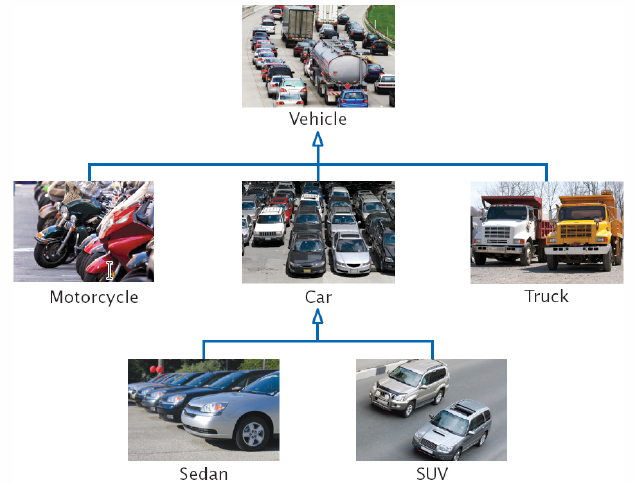
\includegraphics[height=0.55\paperheight]{pucrs-ec-poo-unidade_13-heranca-laminas-heranca.png}\\
	\tiny{Fonte: Java For EveryOne (HORSTMANN, p. 456)}
\end{figure}
\end{column}
\begin{column}{0.55\linewidth}
\begin{itemize}
	\item Se X é subclasse de Y, então Y é superclasse de X e todo X é Y
	\item As classes que herdam características de outras são ditas classes filhas, classes derivadas ou subclasses
	\item As classes a partir das quais outras são derivadas são ditas classes pai ou superclasses
	\item Uma hierarquia de classes pode ter vários níveis
	\item Em uma mesma hierarquia uma classe pode ser considerada superclasse em relação a uma classe e subclasse em relação à outra
\end{itemize}
\end{column}
\end{columns}
\end{frame}

%=======================================================
\section{Exercício}

%-------------------------------------------------------
\begin{frame}\frametitle{Exercício}
Identifique a \textbf{superclasse} e a \textbf{subclasse} em cada um dos seguintes pares de classes:
\begin{itemize}
	\item Empregado x Gerente
\pause
	\begin{itemize}
		\item Superclasse = Empregado / Subclasse = Gerente
	\end{itemize}
	\item EstudanteDeGraduacao x Estudante
\pause
	\begin{itemize}
		\item Superclasse = Estudante / Subclasse = EstudanteDeGraduacao
	\end{itemize}
	\item Pessoa x Estudante
\pause
	\begin{itemize}
		\item Superclasse = Pessoa / Subclasse = Estudante
	\end{itemize}
	\item Empregado x Professor
\pause
	\begin{itemize}
		\item Superclasse = Empregado / Subclasse = Professor
	\end{itemize}
	\item ContaBancaria x ContaComChequeEspecial
\pause
	\begin{itemize}
		\item Superclasse = ContaBancaria / Subclasse = ContaComChequeEspecial
	\end{itemize}
	\item Carro x Veiculo
\pause
	\begin{itemize}
		\item Superclasse = Veiculo / Subclasse = Carro
	\end{itemize}
	\item Veiculo x Caminhao
\pause
	\begin{itemize}
		\item Superclasse = Veiculo / Subclasse = Caminhao
	\end{itemize}
\end{itemize}
\end{frame}

%=======================================================
\section{Exemplo}

%-------------------------------------------------------
\begin{frame}\frametitle{Exemplo}
\begin{itemize}
	\item A Universidade XYZ trabalha com dois tipos de alunos: Regular e Financiado
	\item \textbf{\texttt{AlunoRegular}}
	\begin{itemize}
		\item Custo da mensalidade é baseado no curso/semestre que está cursando, bem como no número da parcela.
		\item São 6 parcelas por semestre, sendo que as 3 primeiras custam 20\% a mais que as demais (fazendo o papel de matrícula).
	\end{itemize}
	\item \textbf{\texttt{AlunoFinanciado}}
	\begin{itemize}
		\item Não paga mensalidade durante o curso. Começará a pagar após o término do mesmo.
		\item A qualquer momento pode consultar seu saldo devedor. Este é calculado tendo por base o curso/semestre em que se encontra e o ano de ingresso na Instituição.
	\end{itemize}
\end{itemize}
\end{frame}

%-------------------------------------------------------
\begin{frame}\frametitle{Exemplo}
\begin{figure}[h]
	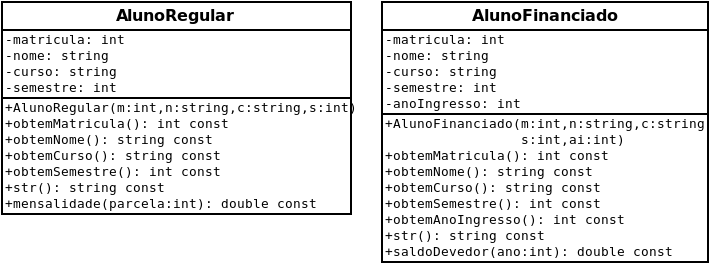
\includegraphics[height=0.45\paperheight]{pucrs-ec-poo-unidade_13-heranca-laminas-exemplo_aluno.png}
\end{figure}
\begin{itemize}
	\item As duas classes \textbf{têm atributos e métodos iguais}!
	\item Se há \textbf{código redundante}, a manutenção será problemática, pois a probabilidade de fazer uma alteração em uma
das classes e esquecer de fazer a mesma alteração na outra é grande
\end{itemize}
\end{frame}

%-------------------------------------------------------
\begin{frame}\frametitle{Exemplo: Herança}
\begin{itemize}
	\item As classes \textbf{\texttt{AlunoRegular}} e \textbf{\texttt{AlunoFinanciado}} podem ser entendidas como um tipo especializado da classe Aluno
	\item Pois compartilham as características comuns a todos os tipos de alunos, porém possuem algumas características a mais que
particularizam sua categoria ou classe
	\item É necessário encontrar uma forma de expressar que certas classes \textbf{compartilham} características (\textbf{atributos} e \textbf{métodos}) com outras
\end{itemize}
\end{frame}

%-------------------------------------------------------
\begin{frame}\frametitle{Exemplo: Herança}
\begin{figure}[h]
	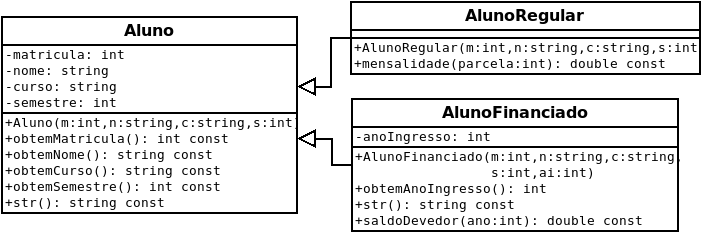
\includegraphics[height=0.45\paperheight]{pucrs-ec-poo-unidade_13-heranca-laminas-exemplo_aluno_com_heranca.png}
\end{figure}
\begin{itemize}
	\item \textbf{\texttt{AlunoRegular}} e \textbf{\texttt{AlunoFinanciado}} estendem \textbf{\texttt{Aluno}}
	\item \textbf{\texttt{AlunoRegular}} e \textbf{\texttt{AlunoFinanciado}} herdam atributos e métodos de \textbf{\texttt{Aluno}}
	\item Logo, o objeto instanciado ``carrega'' todos atributos e métodos
\end{itemize}
\end{frame}

%-------------------------------------------------------
\begin{frame}[fragile]\frametitle{Exemplo: Herança}
\begin{itemize}
	\item Note que as propriedades comuns dos dois tipos de alunos foram concentradas em uma classe chamada \textbf{\texttt{Aluno}}
	\item Diz-se, então, que as classes \textbf{\texttt{AlunoRegular}} e \textbf{\texttt{AlunoFinanciado}} herdam as propriedades
(atributos e métodos) de \textbf{\texttt{Aluno}} e acrescentam suas próprias propriedades a essa descrição
	\item Observe os exemplos de construção dos dois objetos a seguir:
\begin{lstlisting}[language=C++,basicstyle=\ttfamily\small]
AlunoRegular    ar(100001,"Beatriz Silva","4/600",8);
AlunoFinanciado af(100002,"Augusto Alcantara","4/450",6,2018);
\end{lstlisting}
\end{itemize}
\end{frame}

%-------------------------------------------------------
\begin{frame}[fragile]\frametitle{Exemplo: Aluno.hpp}
\lstinputlisting[basicstyle=\ttfamily\tiny]{src/alunos/Aluno.hpp}
\end{frame}

%-------------------------------------------------------
\begin{frame}[fragile]\frametitle{Exemplo: Aluno.cpp}
\lstinputlisting[basicstyle=\ttfamily\tiny]{src/alunos/Aluno.cpp}
\end{frame}

%-------------------------------------------------------
\begin{frame}[fragile]\frametitle{Exemplo: AlunoRegular.hpp}
\lstinputlisting{src/alunos/AlunoRegular.hpp}
\end{frame}

%-------------------------------------------------------
\begin{frame}[fragile]\frametitle{Exemplo: AlunoRegular.cpp}
\lstinputlisting[basicstyle=\ttfamily\scriptsize]{src/alunos/AlunoRegular.cpp}
\end{frame}

%-------------------------------------------------------
\begin{frame}[fragile]\frametitle{Exemplo: AlunoFinanciado.hpp}
\lstinputlisting{src/alunos/AlunoFinanciado.hpp}
\end{frame}

%-------------------------------------------------------
\begin{frame}[fragile]\frametitle{Exemplo: AlunoFinanciado.cpp}
\lstinputlisting[basicstyle=\ttfamily\tiny]{src/alunos/AlunoFinanciado.cpp}
\end{frame}

%-------------------------------------------------------
\begin{frame}[fragile]\frametitle{Exemplo: main.cpp}
\lstinputlisting[basicstyle=\ttfamily\scriptsize]{src/alunos/main.cpp}
\end{frame}

%=======================================================
\section{Lista de Exercícios}

%-------------------------------------------------------
\begin{frame}[fragile]\frametitle{Exercício 1}
\begin{enumerate}
	\setItemnumber{1}
	\item Considere a solução para o exercício 1 proposto na aula sobre ``Makefile e Princípios de POO'' (Livraria), e reimplemente-o para que ele tenha suporte a Herança, tornando-o assim mais simples e evitando códigos redundantes.
\end{enumerate}
\end{frame}

%-------------------------------------------------------
\begin{frame}[fragile]\frametitle{Exercício 2}
\begin{enumerate}
	\setItemnumber{2}
	\item Crie uma hierarquia de classes para representar pessoas, alunos e professores:
	\begin{enumerate}[a.]
		\item Uma pessoa tem um nome e um RG.
		\item Um aluno tem os mesmos atributos que uma pessoa, mas também tem um número de matrícula e um ano de ingresso.
		\item Um professor tem os mesmos atributos que uma pessoa, mas também tem uma unidade (``EP'' para Escola Politécnica, ``EN'' para Escola de Negócios, etc.), um ano de ingresso, e um salário fixo.
	\end{enumerate}
	Crie os métodos básicos de cada classe: construtor, \emph{getters}, \emph{setters} e \texttt{str()}.\\
	Ao final, escreva um programa para testar a hierarquia, criando uma pessoa, um aluno e um professor.
\end{enumerate}
\end{frame}

%-------------------------------------------------------
\begin{frame}[fragile]\frametitle{Exercício 3}
\begin{enumerate}
	\setItemnumber{3}
	\item Um sistema apresenta duas classes:
	\begin{enumerate}[a.]
		\item \texttt{\textbf{ProfessorTI}}: professor de tempo integral, 40 horas, com salário fixo;
		\item \texttt{\textbf{ProfessorH}}: professor horista, com até 20 horas e salário calculado com base no número de horas.
	\end{enumerate}
	As classes são definidas como:
\begin{figure}[h]
	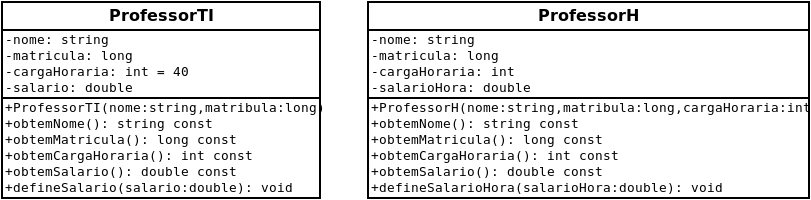
\includegraphics[height=0.35\paperheight]{pucrs-ec-poo-unidade_13-heranca-laminas-exercicio_professor.png}
\end{figure}
\end{enumerate}
\end{frame}

%-------------------------------------------------------
\begin{frame}[fragile]\frametitle{Exercício 3}
\begin{enumerate}
	\setItemnumber{3}
	\item (Continuação)\\
	Ambas têm diversos membros em comum. Então:
	\begin{itemize}
		\item Crie uma classe \texttt{\textbf{Professor}} com o que há de comum entre \texttt{\textbf{ProfessorTI}} e \texttt{\textbf{ProfessorH}};
		\item Redefina \texttt{\textbf{ProfessorTI}} e \texttt{\textbf{ProfessorH}} como subclasses da classe \texttt{\textbf{Professor}};
		\item Implemente as três classes e um programa de teste.
	\end{itemize}
\end{enumerate}
\end{frame}

%=======================================================
\section{Créditos}

%-------------------------------------------------------
\begin{frame}\frametitle{Créditos}
\begin{itemize}
	\item Estas lâminas contêm trechos de materiais disponibilizados pelos professores Rafael Garibotti, Matheus Trevisan, Daniel Callegari, Sandro Fiorini e Bernardo Copstein.
\end{itemize}
\end{frame}

%=======================================================
\section{Soluções}

%-------------------------------------------------------
\begin{frame}[fragile]\frametitle{Exercício 1: Makefile}
\fontsize{3pt}{5pt}\selectfont{
\lstinputlisting{src/livraria/Makefile}
}
\end{frame}

%-------------------------------------------------------
\begin{frame}[fragile]\frametitle{Exercício 1: Promocao.hpp}
\lstinputlisting[basicstyle=\ttfamily\tiny]{src/livraria/Promocao.hpp}
\end{frame}

%-------------------------------------------------------
\begin{frame}[fragile]\frametitle{Exercício 1: Promocao.cpp}
\fontsize{3pt}{5pt}\selectfont{
\lstinputlisting{src/livraria/Promocao.cpp}
}
\end{frame}

%-------------------------------------------------------
\begin{frame}[fragile]\frametitle{Exercício 1: Produto.hpp}
\lstinputlisting[basicstyle=\ttfamily\tiny]{src/livraria/Produto.hpp}
\end{frame}

%-------------------------------------------------------
\begin{frame}[fragile]\frametitle{Exercício 1: Produto.cpp}
\fontsize{3pt}{5pt}\selectfont{
\lstinputlisting{src/livraria/Produto.cpp}
}
\end{frame}

%-------------------------------------------------------
\begin{frame}[fragile]\frametitle{Exercício 1: ProdutoComPaginas.hpp}
\lstinputlisting[basicstyle=\ttfamily\scriptsize]{src/livraria/ProdutoComPaginas.hpp}
\end{frame}

%-------------------------------------------------------
\begin{frame}[fragile]\frametitle{Exercício 1: ProdutoComPaginas.cpp}
\lstinputlisting[basicstyle=\ttfamily\tiny]{src/livraria/ProdutoComPaginas.cpp}
\end{frame}

%-------------------------------------------------------
\begin{frame}[fragile]\frametitle{Exercício 1: ProdutoComPaginasEAno.hpp}
\lstinputlisting[basicstyle=\ttfamily\tiny]{src/livraria/ProdutoComPaginasEAno.hpp}
\end{frame}

%-------------------------------------------------------
\begin{frame}[fragile]\frametitle{Exercício 1: ProdutoComPaginasEAno.cpp}
\fontsize{3pt}{5pt}\selectfont{
\lstinputlisting{src/livraria/ProdutoComPaginasEAno.cpp}
}
\end{frame}

%-------------------------------------------------------
\begin{frame}[fragile]\frametitle{Exercício 1: app.cpp}
\fontsize{3pt}{5pt}\selectfont{
\lstinputlisting{src/livraria/app.cpp}
}
\end{frame}

%-------------------------------------------------------
\begin{frame}[fragile]\frametitle{Exercício 2: Makefile}
\lstinputlisting[basicstyle=\ttfamily\tiny]{src/professor_aluno/Makefile}
\end{frame}

%-------------------------------------------------------
\begin{frame}[fragile]\frametitle{Exercício 2: Pessoa.hpp}
\lstinputlisting[basicstyle=\ttfamily\tiny]{src/professor_aluno/Pessoa.hpp}
\end{frame}

%-------------------------------------------------------
\begin{frame}[fragile]\frametitle{Exercício 2: Pessoa.cpp}
\fontsize{3pt}{5pt}\selectfont{
\lstinputlisting{src/professor_aluno/Pessoa.cpp}
}
\end{frame}

%-------------------------------------------------------
\begin{frame}[fragile]\frametitle{Exercício 2: Aluno.hpp}
\lstinputlisting[basicstyle=\ttfamily\tiny]{src/professor_aluno/Aluno.hpp}
\end{frame}

%-------------------------------------------------------
\begin{frame}[fragile]\frametitle{Exercício 2: Professor.cpp}
\fontsize{3pt}{5pt}\selectfont{
\lstinputlisting{src/professor_aluno/Professor.cpp}
}
\end{frame}

%-------------------------------------------------------
\begin{frame}[fragile]\frametitle{Exercício 2: Professor.hpp}
\lstinputlisting[basicstyle=\ttfamily\tiny]{src/professor_aluno/Professor.hpp}
\end{frame}

%-------------------------------------------------------
\begin{frame}[fragile]\frametitle{Exercício 2: Aluno.cpp}
\fontsize{3pt}{5pt}\selectfont{
\lstinputlisting{src/professor_aluno/Aluno.cpp}
}
\end{frame}

%-------------------------------------------------------
\begin{frame}[fragile]\frametitle{Exercício 2: app.cpp}
\lstinputlisting[basicstyle=\ttfamily\scriptsize]{src/professor_aluno/app.cpp}
\end{frame}

%-------------------------------------------------------
\end{document}
	
